\documentclass[a4paper
,oneside,11pt]{article}
\usepackage[french]{babel}
\usepackage[utf8]{inputenc}
\usepackage[french]{babel}
\usepackage{fullpage}
\usepackage{xkeyval}
\usepackage{rotating}
\usepackage{amsmath}
\usepackage{amsfonts,amssymb}
\usepackage{float}
\usepackage{fancyhdr}
\usepackage{graphicx}
\usepackage{verbatim}
\usepackage{lastpage}
\usepackage{pstricks}
%\usepackage{aeguill}
\usepackage{color}
\usepackage{multicol}
\usepackage{mathenv}
\usepackage{amssymb}
\setlength{\headsep}{0.70cm}

%%%%%%%%%%%%%%%% Variables %%%%%%%%%%%%%%%%
\def\titre{Rapport\\Projet de Fin d'Année :\\Braille Music Compiler}
\def\titregauche{Projet de Fin d'Année}
\def\titredroite{Rapport de projet}
\def\filiere{informatique}
\def\annee{$2^{eme}$}  % $1^{ere}$, $2^{eme}$ ou $3^{eme}$
\def\anneescolaire{2011/2012}
\def\equipe{Pierrick Baudet \\ Pierre-Yves Canneill \\ David Dallago \\ Lun Jiang \\ Benjamin Lux \\Sara Rahhali\\Ali Slimani Houti}
\def\encadrant{Vinh-Thong Ta}
%%%%%%%%%%%%%%%%%%%%%%%%%%%%%%%%%%%%%%%%%%%


\pagestyle{fancy} \lhead{\textsc{\titregauche}} 
\rfoot{\textit{Ann\'ee \anneescolaire}}\rhead{\textsc{\titredroite}}\cfoot{\thepage/\pageref{LastPage}}
\renewcommand{\headrulewidth}{0.4pt}
\renewcommand{\footrulewidth}{0.4pt}

\newcommand{\HRule}{\rule{\linewidth}{0.5mm}}

\begin{document}

\begin{titlepage}

\begin{center}


% Upper part of the page
\begin{center}
\rotatebox{0}{\scalebox{1}[1]{
\includegraphics[width=5cm]{images/Logo_ENSEIRB-MATMECA.png}}}
\end{center}
~\\
~\\
~\\
\textsc{\LARGE ENSEIRB-MATMECA}\\[1cm]

\textsc{\Large {Fili\`ere \filiere, \annee ann\'ee}}\\[0.5cm]

% Title
\HRule \\[0.4cm]
{ \huge \bfseries \titre}\\[0.4cm]


\HRule \\[1.5cm]


% Author and supervisor
\begin{minipage}{0.4\textwidth}
\begin{flushleft} \large
\emph{Auteurs:}\\
\equipe
\end{flushleft}
\end{minipage}
\begin{minipage}{0.4\textwidth}
\begin{flushright} \large
\emph{Encadrant:} \\
\encadrant
\end{flushright}
\end{minipage}


\vfill

% Bottom of the page
{\large \today}

\end{center}

\end{titlepage}
\tableofcontents\thispagestyle{fancy}
\newpage
\section*{Introduction}\thispagestyle{fancy}
\addcontentsline{toc}{section}{Introduction}
\subsection*{Contexte}
Braille Music Compiler (BMC) est un outil de conversion du braille musical principalement destiné à l'usage de personnes aveugles ou malvoyantes. Il est capable d'interpréter une partition écrite en braille pour la convertir en une sortie audio qui peut par la suite être transformée en un fichier  MIDI ou MusicXML.\\

  BMC est actuellement à l'état de prototype, il est en cours de développement par Mario Lang, un autrichien non-voyant passionné par la musique et l'informatique.

  L'idée de développer un tel outil lui est venue lorsqu'il voulu jouer des partitions braille de musique classique. Souvent, il n'était pas sûr de bien interpréter certaine notes et s'est vite rendu compte que cette notation peut parfois porter à confusion. La notation Braille musicale est, en effet, assez complexe et peut parfois sembler ambiguë d'où l'utilité d'un programme qui servirait de référence en permettant d'écouter la note jouée. 
  
  Seulement la plupart des programmes disponibles sur le marché qui vont dans ce sens sont assez chers - coût moyen de 600 euros - et ne sont en général compatibles qu'avec Windows, ce qui limite fortement leur utilisation.\\
 
  M. Lang commença par travailler sur \textit{FreeDots}, un programme capable de convertir des partitions \textit{noires} de musique en partitions braille.\\
  Encouragé par le succès que rencontra ce premier programme, Il décida ensuite de se lancer dans la transcription inverse du braille musical, ce qui donna naissance au Braille Music Compiler. \\
  
  L'amélioration de l'utilisation du BMC notamment par implémentation d'une interface graphique nous a alors été proposée par Samuel Thibault, chercheur à l'INRIA et proche collaborateur du développeur du BMC. 
  
  
 
\subsection*{Problématique}
Le Braille Music Compiler est, pour l'instant, toujours en cours de développement. En effet, l'exécution de sa version actuelle requiert une certaine connaissance des outils informatiques, chose qui rend difficile son utilisation par un usager lambda.\\
L'intérêt de ce projet est donc d'améliorer cet outil de façon à ce qu'il devienne accessible à un plus large public. La mise en oeuvre d'une interface graphique permettrait en effet de rendre son utilisation plus intuitive.\\

  Étant principalement dédié à l'usage de personnes non(ou mal)-voyantes, l'interface graphique à implémenter doit donc répondre à un certain nombre de critères en termes d'accessibilité, elle doit être simple mais fonctionnelle.
  De plus, il serait intéressant que cette interface comporte aussi des fonctionnalités d'édition et de modifications de fichiers écrits en braille musical.
   
  Le BMC a aussi pour ambition de faciliter la collaboration entre voyants et non-voyants, en ce sens, l'interface devrait pouvoir à la fois afficher les partitions de musique écrites en braille et en \textit{noir} permettant ainsi à chacun des collaborateurs de pouvoir se repérer par rapport aux partitions de l'autre.    



\section{Organisation du travail}
%% Organisation du travail
\subsection{Méthode Scrum}
%% importance des tâches/ périodes de 3 semaines / selection des tâches / encadrant pédagogique
Le responsable pédagogique de ce pfa, monsieur Ta, a préféré au classique cahier des charges une utilisation des méthodes agiles, plus précisément de la méthode \textit{scrum}.  Cette méthode semble être efficace puisque nous avons aujourd'hui atteint en grande partie nos objectifs. En effet, malgré des périodes de bas régime, les dates de rendus périodiques entraînent un certain rythme. Enfin, cette méthode nous prépare à l'entreprise puisque de nos jours, la plupart d'entre elles utilisent cette méthode.



\subsubsection*{Le Product Backlog}
La méthode \textit{scrum} place tous les collaborateurs du projet sur un pied d'égalité. Il faut tout d'abord créer un Product Backlog qui correspond à toutes les tâches à effectuer jusqu'à la finalisation du projet.
Ce document doit être validé avec le client, puis ce dernier attribue des notes aux tâches, aboutissant à un ordre de priorité.

\subsubsection*{Un Sprint Backlog}
Ces dernières sont ensuite réparties en Sprint Backlog. Ce sont des périodes courtes (quelques semaines) durant lesquelles l'équipe travaille sur certaines tâches définies au départ. Nous avons découpé notre Product Backlog en 4 Sprints.
À la fin de chaque Sprint, l'équipe présente sont travail sous forme concrète au client, sous forme d'un exécutable, de maquettes ou toute autre forme.
Ceci est fait pour éviter au projet de partir dans une mauvaise direction et permet au client, dont les envies peuvent varier, de prendre part activement au projet.
La fin d'un Sprint laisse place à une nouvelle réunion où sont définis les objectifs du Sprint suivant.

\subsubsection*{Les moyens de communication}
Afin de pouvoir travailler de façon efficace en groupe, il est nécessaire de disposer d'outils spécialisés dans la gestion de projet.
Nous avons mis en place trois de ces outils.
Pour faciliter la communication au sein du groupe nous avons créé la mail-liste \textit{pfa.bmc@listes.enseirb-matmeca.fr}. Cette liste est utilisable par tout le monde (membres du groupe, client, résponsable pédagogique) et redirige vers les membres du groupe.
Pour gérer la méthode \textit{scrum} nous communiquons via une collection \textit{Google docs} qui se compose essentiellement du Product Backlog, du détail des Sprint Backlog, du compte-rendu des réunions avec l'encadrant et d'un tableau blanc.
Enfin nous avons mis en place un répertoire de travail sur \textit{Github} accessible en écriture aux membres du projet et visible par tous. Celui-ci est accessible à l'adresse \textit{https://github.com/ddallago/pfa.bmc}.



%\section{Spécification des besoins}
\section{Interfaces Graphiques}
Lors du développement de ce projet, l'accessibilité était un argument essentiel à prendre compte dans les choix d'implémentation. Ainsi, nous n'avons pas élu la bibliothèque graphique \textit{Qt}, car bien qu'adaptée à plusieurs systèmes d'exploitation, elle risquait de poser certains problèmes de compatibilité pour des utilisateurs non-voyant se servant de lecteurs d'écran.  
%L'un des critères essentiels de ce projet est l'accessibilité. Ce qui fait que nous n'avons pas pu utilisé une bibliothèque graphique cross-platform comme Qt, car ce type de bibliothèque a des prolèmes de compatibilité avec les lecteurs d'écran des systèmes d'exploitation. 
Avec les suggestions du M. Lang et celles de M.Thibaut, les bibliothèques graphiques \textit{GTK+} sous Linux et \textit{Winforms} sous Windows ont ainsi été privilégiées.

\subsection{Unix}
% unix.tex


\subsection{Windows}
% windows.tex





\section{Back-end de \textit{BMC}}
\subsection{Langage Abstrait de \textit{BMC}}

\textit{Braille music compiler} est un programme qui a pour objectif
de transformer un fichier écrit en \textit{Braille Music} en un autre
langage utilisable par d'autres applications. La difficulté est que le
langage \textit{Braille Music} possède beaucoup d'ambiguïtés, en effet
par exemple pour connaître la note exacte en cours, il est nécessaire
de savoir quelles ont été les notes précédentes. \`A l'heure actuelle
le programme arrive correctement à compiler le langage \textit{Braille
  Music} en un langage Abstrait qui lui ne possède aucune
ambiguïté. Ce langage abstrait peut être converti en n'importe quels
formats de musique. Par exemple :

\begin{itemize}
\item MIDI (Format AUDIO)
\item MusicXML 
\item lilypond (Equivalent au Latex, mais pour la musique)
\end{itemize}
Le schéma \ref{compiler} résume le fonctionement de BMC.

\begin{figure}[!h]
  \centering
  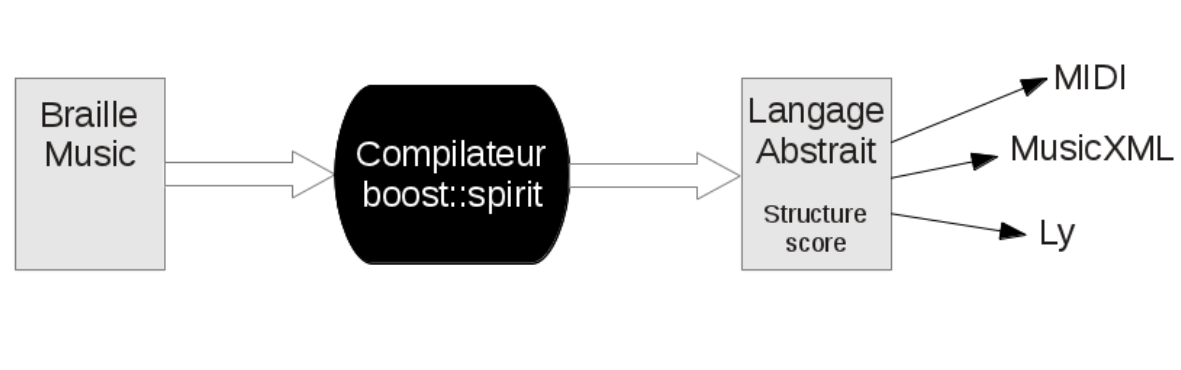
\includegraphics[width=1\textwidth]{images/fonction-bmc.png}
  \caption{Schéma visuel du fonctionement de BMC}
  \label{compiler}
\end{figure}

Notre travail a été d'implémenter quelque uns de ces modules de
conversion. Pour cela il est nécessaire de comprendre comment est
conçu le langage Abstrait. Après la compilation du \textit{Braille
  Music}, l'ensemble des données sont stockées dans une structure
nommée "score". Cette structure est une multitude de vecteurs
imbriqués les uns dans les autres. Voici le code de la strucure suivi
d'une représentation visuel (\ref{score}) :

\begin{verbatim}
typedef boost::variant<note, rest, chord, value_distinction, hand_sign, simile, barline>;
typedef std::vector<sign> partial_voice;
typedef std::vector<partial_voice> partial_measure;
typedef std::vector<partial_measure> voice;
struct measure : locatable
{
  boost::optional<unsigned> ending;
  std::vector<voice> voices;
};
typedef std::vector< boost::variant<measure> > staff;
typedef std::vector<staff> part;
struct score {
  boost::optional<time_signature> time_sig;
  std::vector<part> parts;
};
\end{verbatim}

\begin{figure}[h]
  \centering
  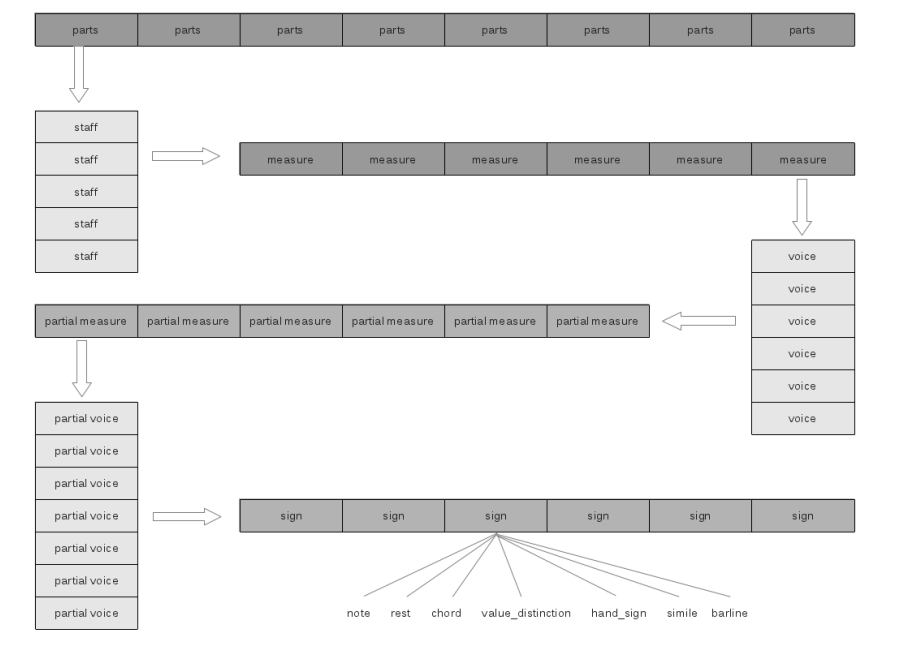
\includegraphics[width=1\textwidth]{images/bmc-score.png}
  \caption{Représentation de la structure score}
  \label{score}
\end{figure}

Il est donc maintenant plus facile d'expliquer la structure
\textit{score}. Un fichier de musique braille peut donc se diviser en
plusieurs parties (parts). Chaque partie possède un ou plusieurs
"staff". Un "staff" n'est autre que la portée, typiquement si le
compositeur écrit une partition de musique pour piano il y aura deux
portées. Chaque portée possède un nombre de mesures. Si la musique
composée est polyphonique il y aura plusieurs voix ("voices"). Une
voix est ensuite divisée en mesures partielles, ces mesures partielles
pouvant de nouveau être divisées en voix ("partial\_voices") qui elles
sont divisées en un vecteur de \textit{sign}. Un sign pouvant être une
note, un repos, une barre ... La figure \ref{musicexe} représente sur
une partition de musique ses différents termes.


\begin{figure}[!h]
  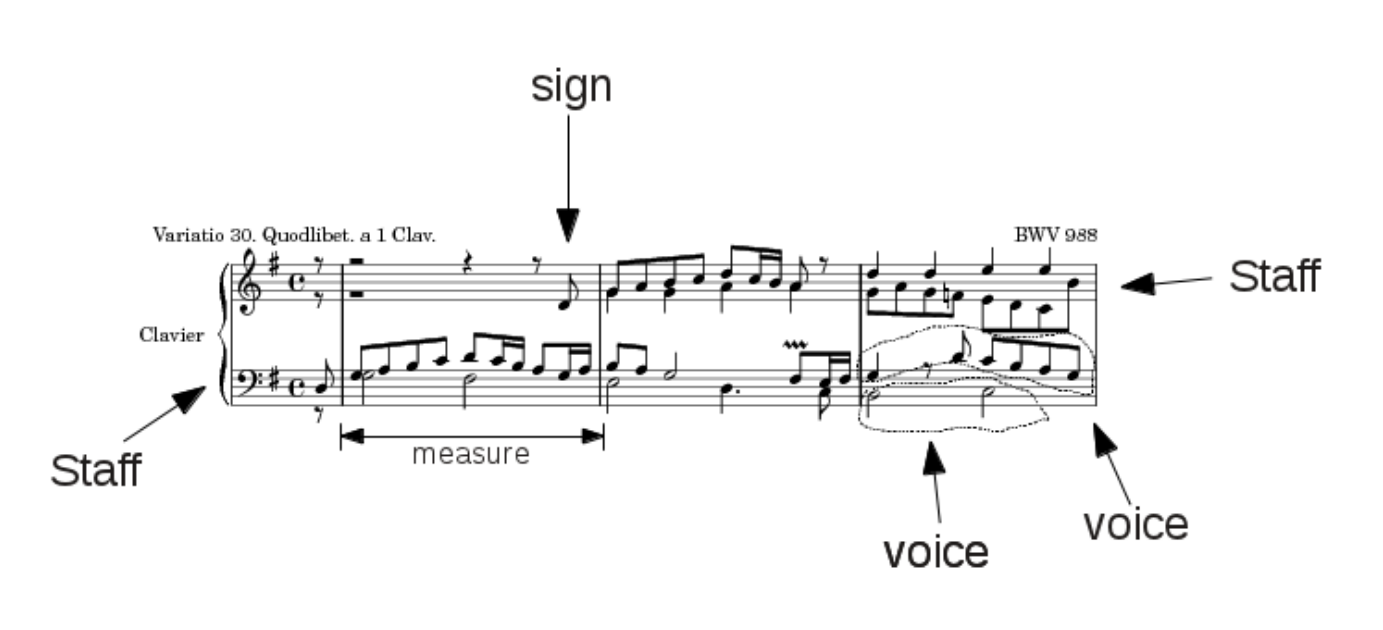
\includegraphics[width=1\textwidth]{images/score-visu.png}
  \caption{Un petit exemple visuel}
  \label{musicexe}
\end{figure}

À partir de ce langage intermédiaire nous avons pu réaliser deux
classes qui ont été intégré dans le programme bmc. Chaqu'une d'elle
créer un fichier représentant une partition braille passée en argument
dans un autre langage.




\subsection{Sortie Lilypond}
% lilypond.tex

% ben : je veux bien m'en charger
\subsubsection{Génération du fichier Lilypond}
Nous nous somme dans un premier temps consacré à l'exportation sous le
format lilypond.  Ce format est destiné à produire des partitions au
format pdf de grande qualité.  Ce choix nous est apparut fondamental,
d'une part le format pdf est très répandu, d'une autre cela nous a
permit de pouvoir afficher la partition pour voyant dans notre
interface graphique.

L'implémentation de cette fonctionalité consiste en la création de la
classe \textit{toLily}. Les fonctions de cette classe parsent le
langage abstrait produit par le \textit{BMC} pour le convertir en langage
lilypond. Ce dernier ressemble un peu au langage \LaTeX. À chaque
structure contenue dans le premier langage on associe une action qui
écrira dans le fichier lilypond généré et mettra à jour les variables
de la classe.

Une fois cette classe implémenté nous l'avons partagé avec M Lang. Il
l'a ensuite amélioré avant de l'intégrer dans \textit{BMC}.


\subsubsection{Génération du format pdf}
Une fois le fichier lilypond généré par cette nouvelle version de \textit{BMC}
crée, il est facile d'obtenir un pdf de la partition correspondante à
l'aide de la commande : $$lilypond\ fichier.ly$$ Cependant nous
avions besoin dans notre interface graphique de récupérer certaines
informations lorsque l'utilisateur clique sur les notes de ce pdf.

Lors de la construction du pdf le logiciel lilypond ce charge de
rajouter des liens des notes vèrs la note correspondante dans le
fichier \textit{.ly}. Nous avons crée un programme pour remplacer ces
liens par les informations souhaitées ,\textit{i.e.} la position de la
note dans le fichier \textit{braille music}. Après avoir rajouté en commentaire
ces informations après chaque note dans le fichier lilypond, ce
programme compile d'abord le fichier en format ps grace à la commande
$$lilypond\ --ps\ fichier.ly$$ Puis il remplace tous les liens
vèrs le fichier lilypond par la position de la note dans le fichier
\textit{braille music}, enfin il compile le ps obtenue en pdf grace à la
commade : $$ps2pdf\ fichier.ps$$

Le pdf obtenu est ensuite utilisable par notre interface graphique.


\subsection{Sortie MIDI}
% midi.tex
\subsubsection{Le format de fichier MIDI}
Le format MIDI est assez simple à résumer. Il comporte un ensemble fini d'entiers compris entre 0 et 127 représentant la note que l'on entend. Chaque octave est composée de douze tonalités comme indiqué dans la Figure \ref{midiNote}.  
\begin{figure}[h]
\centering
\includegraphics[width=0.5\textwidth]{images/midiNotes.png}
\caption{Notes MIDI}
\label{midiNote}
\end{figure}

La lecture d'un flux MIDI se fait linéairement: le lecteur lit des messages de statut, par exemple NOTE\_ON, et les deux arguments qui suivent, qui correspondent au numéro de note à jouer ainsi que la vélocité d'attaque de la note. La Figure \ref{midiHexa} présente l'aperçu d'un fichier MIDI:
\begin{figure}[h]
\centering
\includegraphics[width=0.5\textwidth]{images/midiHexa.png}
\caption{Fichier MIDI}
\label{midiHexa}
\end{figure}

Dans cet exemple, on peut trouver:
\begin{itemize}
\item \textit{0x90} Message de statut : NOTE\_ON \textit{0x3C} Numéro de note: 60 \textit{0x5F} Vélocité: 90
\item \textit{0x80} Message de statut : NOTE\_OFF \textit{0x3C} Numéro de note: 60 \textit{0x00} Vélocité: 0
\end{itemize}
On notera que la vélocité est de 0 lors d'un message NOTE\_OFF. En effet, la notion de vélocité n'a pas vraiment de sens lorsqu'il s'agit d'arrêter de jouer une note.

\subsubsection{Librairie utilisée}
La librairie à trouver devait répondre à des besoins de bas niveaux que présentait l'objectif de sortie MIDI à partir du fichier braille. En effet, la plupart des librairies existantes portent sur la lecture de flux MIDI. Après maintes recheches, nous avons finalement décidé d'utiliser la libraire SMF (Standard MIDI File format). Le travail a pu démarrer sur l'exportation du format braille vers le MIDI. Il est à noter que la librairie est écrite en C mais que le développeur l'a rendu compatible avec les compilateurs C++ en utilisant le mot clé $extern$ pour le linkage.

\subsubsection{L'exportation}
Deux classes ont été créées afin de réaliser l'exportation:
\begin{itemize}
  \item toMidi ;
  \item keyWithInfo.
\end{itemize}

La classe \textit{toMidi} sert à redéfinir les opérateurs () de la même façon que ce qui a été fait pour l'exportation au format \textit{Lilypond}, avec bien entendu des différences dans le traitement.
La classe \textit{keyWithInfo} est celle qui contient l'information nécessaire à l'exportation:
\begin{verbatim}
class noteWithInfo{
  public:
     braille::ambiguous::note *note;
     int accidental;
     double start_date;
     double end_date;
     bool begin_repeat;
     bool end_repeat;
     int nb_repetitions;
};
\end{verbatim}
Le champ \textit{note} provient de la structure de M.Lang. Il contient les informations quant à l'octave, le numéro de la note, la durée (par l'utilisation de méthodes que M.Lang a créées). Le champ \textit{accidental} correspond au nombre de dièses ou de bémols qu'il y a devant la note.
Enfin, les champs les plus interessants sont les derniers: \textit{start\_date} et \textit{end\_date} correspondent à la date de départ de la note et celle de sa fin, en temps absolu. Les champs \textit{begin\_repeat} et \textit{end\_repeat} sont des booléens qui indiquent si on a un debut de zone de répétition ou de fin de zone de répétition. Enfin, le champs \textit{nb\_repetitions} correspond au nombre de fois que la zone repérée doit être répétée. 

Le parcours de la structure abstraite de M.Lang  est donc effectué et stocke des pointeurs vers des objets de type \textit{noteWithInfo} dans le champs $std::list<noteWithInfo*>song[2]$ de la classe \textit{toMidi}. On notera que \textit{song} est donc un tableau de deux listes contenant des pointeurs vers des \textit{noteWithInfo} afin de représenter les notes contenues dans une partition à deux clés commes les partitions pour piano par exemple. Il sera facile pour le client de paramétrer cette valeur, le parcours réalisé étant générique.

\subsubsection{L'enregistrement}
Une fois le tableau de listes rempli, on se sert des primitives de la librairies \textit{smf} afin de créer la note MIDI correspondant à chaque cellule. Les primitives de la librairies permettent alors d'écrire dans un fichier les messages ainsi créés. Le traitement étant générique, l'enregistrement marchepour des partitions à deux clés mais tout autant que pour plus ou moins. Deux méthodes ont été mises en place à cette fin:
\begin{itemize}
\item $void toMidi::unfold\_ repetitions()$ ;
\item $void toMidi::generate\_ midi\_ file()$.
\end{itemize}
La méthode $unfold\_ repetitions$ est nécessaire car la librairie n'a pas de fonctionnalité gérant les répétitions. Il a donc été nécessaire de recopier les zones à répéter dans la liste en prenant en compte les temps de démarrage et de fin. 
La méthode $generate\_ midi\_ file$ est celle qui parcourt le tableau de listes \textit{song} et qui utilise les fonctions de la librairies SMF afin de générer le fichier \textit{midi}.




\section{Objectifs/Travail restant}
% objectifs.tex

\subsection{Portage sous Windows}

\subsection{GUI sous MacOs}

\subsection{Autres formats de sortie pour bmc}

\subsection{Autres fonctionnalitées du gui}



\section*{Conclusion}\thispagestyle{fancy}
\addcontentsline{toc}{section}{Conclusion}

\chapter{Conclusion}

Ce premier rapport ainsi que le \textbf{Product Backlog} en annexe résultent des différents rendez-vous avec le client local ainsi que les multiples réunions que l'équipe a eu avec l'encadrant pédagogique.\\
Ces deux documents font état de l'avancement du projet à ce jour.\\

La réalisation du projet étant amenée à avancer, certains points de ce document sont susceptibles d'être modifiés. Cependant, les points fondamentaux de la conception du projet se doivent d'être respectés.\\




%\section{Glossaire}
%%%


\end{document}

